\epi{“对此感兴趣,并且希望做点什么。”}
{\textit{在为 Go 添加复数支持时}\\ \textsc{KEN THOMPSON}}

\noindent{}什么是 Go?来自于网站:\cite{go_web}:
\begin{quote}
Go 编程语言是一个使得程序员更加有效率的开源项目。Go 是有表达力、简洁、清晰和有效率的。
它的并行机制使其很容易编写多核和网络应用,而新奇的类型系统允许构建有弹性的模块化程序。
Go 编译到机器码非常快速,同时具有便利的垃圾回收和强大的运行时反射。
它是快速的、静态类型编译语言,但是感觉上是动态类型的,解释型语言。
\end{quote}

Go 是一个年轻的语言,特性仍然在不断增加或\emph{删除}中。
所以当你阅读的时候,可能部分内容已经过时。
一些练习的答案可能会随着 Go 不断的演化而变成错误的。
我们将尽可能让这个文档与最新的 Go 发布版本保持一致。
通过努力已经建立了“特性检验”代码示例。

本书使用了下面的约定:
\begin{itemize}
\item 代码用 \prog{DejaVu Mono} 显示;
\item 关键词用 \key{DejaVu Mono Bold} 显示;
\item 注释用 \rem{DejaVu Mono Italic} 显示;
\item 代码中额外的标记,\coderemark{用这种形式展现};
\item 使用数字 \gocircle{1} 对长内容标记——解释会跟随其后;
\item 行号在右边展示;
\item Shell 示例用 \pr{} 作为标记;
\item 强调的段落会缩进,在左边有竖线。
\end{itemize}

\section{官方文档}
Go 已经有大量的文档。
\gomarginpar{在互联网上搜索时,应当使用“golang”这个词来代替原始的“go”。}
例如 Go Tutorial \cite{go_tutorial} 和 Effective Go \cite{effective_go}。
网站 \url{http://golang.org/doc/} 是绝佳的起点 
\footnote{\url{http://golang.org/doc/} 本身是由 Go 程序 \prog{godoc} 提供服务的。}。
虽然并不一定要阅读这些文档,但是强烈建议这么做。

Go 用叫做 \prog{godoc} 的 Go 程序格式化其文档。
你可以用它查阅在线文档。例如,假设我们需要了解关于 \package{hash} 包的更多信息。
可以用命令 \prog{godoc hash} 查阅它。如何创建你自己的包的文档在第
\ref{chap:packages} 章中介绍。

\section{获得 Go}
Ubuntu 和 Debian 都有 Go 包在其仓库中,查找“golang”包。但是工作的时候仍然有一些小问题。现在仍然使用源码进行安装。

因此将会从 mercurial 中获取代码并且编译。
对于其他类 Unix 系统,过程类似。
\begin{itemize}
\item 首先安装 Mercurial (获取 \prog{hg} 命令)。
在 Ubuntu/Debian/Fedora 需要安装 \prog{mercurial} 包;

\item 为了编译 Go 需要包:\prog{bison},\prog{gcc},\prog{libc6-dev},\prog{ed},\prog{gawk} 和 \prog{make};

\item 设置环境变量 \prog{GOROOT} 为 Go 安装目录:
\begin{display}
\pr \user{export GOROOT=~/go}
\end{display}

\item 然后获取 Go 源代码:
\begin{display}
\pr \user{hg clone -r release https://go.googlecode.com/hg/ $GOROOT}
\end{display}

\item 设置 PATH 到 Go 的二进制文件所在目录,这样 Shell 可以找到它们:
\begin{display}
\pr \user{export PATH=$GOROOT/bin:$PATH}
\end{display}

\item 编译 Go
\begin{display}
\pr \user{cd $GOROOT/src}
\pr \user{./all.bash}
\end{display}
\end{itemize}
如果全部都没问题,你应当看到下面的内容:
\begin{display}
Installed Go for linux/amd64 in /home/go.
Installed commands in /home/go/bin.
The compiler is 6g.
\end{display}
现在,Go 已经被安装到了系统中,可以开始游戏了。

\subsection{保持更新}
新的发布会公布在 Go Nuts 邮件列表 \cite{go_nuts} 中。将已经存在的代码树更新到最新,需要执行:
\begin{display}
\pr \user{cd $GOROOT}
\pr \user{hg pull}
\pr \user{hg update release}
\pr \user{cd src}
\pr \user{./all.bash}
\end{display}
\noindent{}看看你现在用的版本:
\begin{display}
\pr \user{cd $GOROOT}
\pr \user{hg identify}
79997f0e5823 release/release.2010-10-20
\end{display}
\noindent{}这是 \gorelease{2010-10-20} 版本。
\noindent{}这是 \gorelease{2010-10-20} 版本。发布描述为“稳定”发布,相比之下,“weekly”发布就要变化更多一些。
如果希望跟踪 weekly 发布,而不是稳定的版本,可以使用:
\begin{display}
\pr \user{hg update weekly}
\end{display}
代替
\begin{display}
\pr \user{hg update release}
\end{display}

\section{前身}
Go 的前身来自于 Inferno \cite{inferno} (基于 Plan 9 \cite{plan9} 的改造)。
Inferno 包含了一个叫做 Limbo \cite{limbo} 的语言。来自于 Limbo 论文中的引用:
\begin{quote}
Limbo 是用于开发运行在小型计算机上的分布式应用的编程语言。
它支持模块化编程,编译期和运行时的强类型检查,\emph{进程内基于具有类型的 channel 通讯},
原子性\emph{垃圾收集},和简单的抽象数据类型。
它被设计用于即便是没有硬件内存保护的小型设备上,也能安全的运行。
\end{quote}
Limbo 的一个特性已经包含进了 Go 用于支持交叉编译。
Go 从 Limbo 继承的另一个特性是 channel(参阅第 \ref{chap:channels} 章)。
从 Limbo 文档来的另一段:
\begin{quote}
[channel] 是用于向系统中其他代理发送和接收特定类型对象的通讯机制。
channel 可以用于本地进程间通讯;用于连接到命名的目的地的库方法。
两种情况都是直接发送和接收操作的。
\end{quote}
在 Go 中,channel 比在 Limbo 中更加好用。
如果我们对 Go 的历史深入探索,会发现一个到 "Newsqueak" \cite{newsqueak} 的引用,
这是在类 C 语言中使用 channel 通讯的拓荒者。
channel 对于这些语言并不是独一无二的,另一个非类 C 语言,Erlang \cite{erlang},也在使用它。

\begin{figure}[H]
\caption{Go 编年史}
\label{fig:chrono-of-go}
\begin{center}
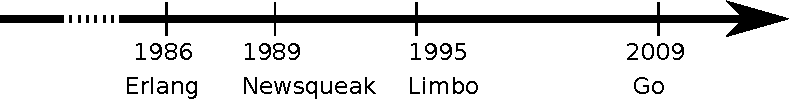
\includegraphics[scale=0.65]{fig/go-history.pdf}
\end{center}
\end{figure}

使用 channel 与其他进程进行通讯的办法,
叫做通讯序列化过程(Communicating Sequential Processes - CSP),
由 C. A. R. Hoare \cite{hoare} 设计构想,而他正是那个发明快速排序 \cite{Quicksort} 算法的人。

\begin{lbar}[]
Go 是第一个实现了简单的(或更加简单的)并行开发的、夸平台类 C 语言。
\end{lbar}

\section{练习}
\begin{Exercise}[title={文档},difficulty=1]
\label{ex:doc}
\Question
Go 的文档可以通过~\prog{go doc} 程序阅读,它包含在~Go 的发布包中。

\prog{go doc hash} 给出了~\package{hash} 包的信息:
\vskip\baselineskip
\begin{display}
\pr \user{go doc hash}
PACKAGE

package hash

...
...
...

SUBDIRECTORIES

        adler32
        crc32
        crc64
        fnv

\end{display}
\vskip\baselineskip
哪个~\prog{go doc} 的命令可以显示~\package{hash} 包中的~\package{fnv} 文档?

\end{Exercise}

\begin{Answer}
\Question
\package{fnv} 包在~\package{hash} 的\emph{子目录}中,所以只需要 
\quad \texttt{go doc hash/fnv} 即可。


所有的内建函数同样可以通过~\prog{godoc} 程序访问:\prog{go doc builtin}。
\end{Answer}


\cleardoublepage
\section{答案}
\shipoutAnswer
